\chapter{Developing Process}

\section{Developer Interaction}

\section{Team Organisation}

\section{CI/CD}
To facilitate the continues integration of new code by all developers, several workflows/pipelines have been implemented to ensure that each pull request (PR) is subjected to various checks, including building, testing, and code quality analysis to mitigate the risk of the service to break. This could happen due to defects, vulnerabilities, and other undesirable coding practices. Once these checks are successfully completed, the PR is deemed safe for merging into the master branch, which initiates a deployment pipeline.

\subsection{build-test.yml}
This workflow performs the build and testing of the entire stack of the service, including the backend and fronted. The pipeline is triggered on push event to any branch and includes two jobs: \\

\textbf{build-test-backend}, which runs on an ubuntu 20.04 machine and includes the following steps:

\begin{enumerate}
    \item Checkout the repository
    \item Set up .NET version 7.0.x
    \item Restore dependencies
    \item Build the MiniTwit backend
    \item Run backend tests
\end{enumerate}

\textbf{build-test-frontend}, which runs on an ubunto 20.04 machine and includes the following steps:

\begin{enumerate}
    \item Checkout the repository
    \item Install Node.js version 18 and dependencies for caching
    \item Install dependencies for the MiniTwit frontend
    \item Build the MiniTwit frontend
    \item Run frontend tests using Playwright, in a docker container started by docker-compose -f docker-compose.ui.yml up -d
    \item Stop the UI service by shutting down the Docker containers created with docker-compose
\end{enumerate}

\subsection{codeql.yml}
Pipeline for codeQL (C sharp) 

\subsection{eslint.yml}
Pipeline for checking TS code

\begin{figure}[H]
    \centering
    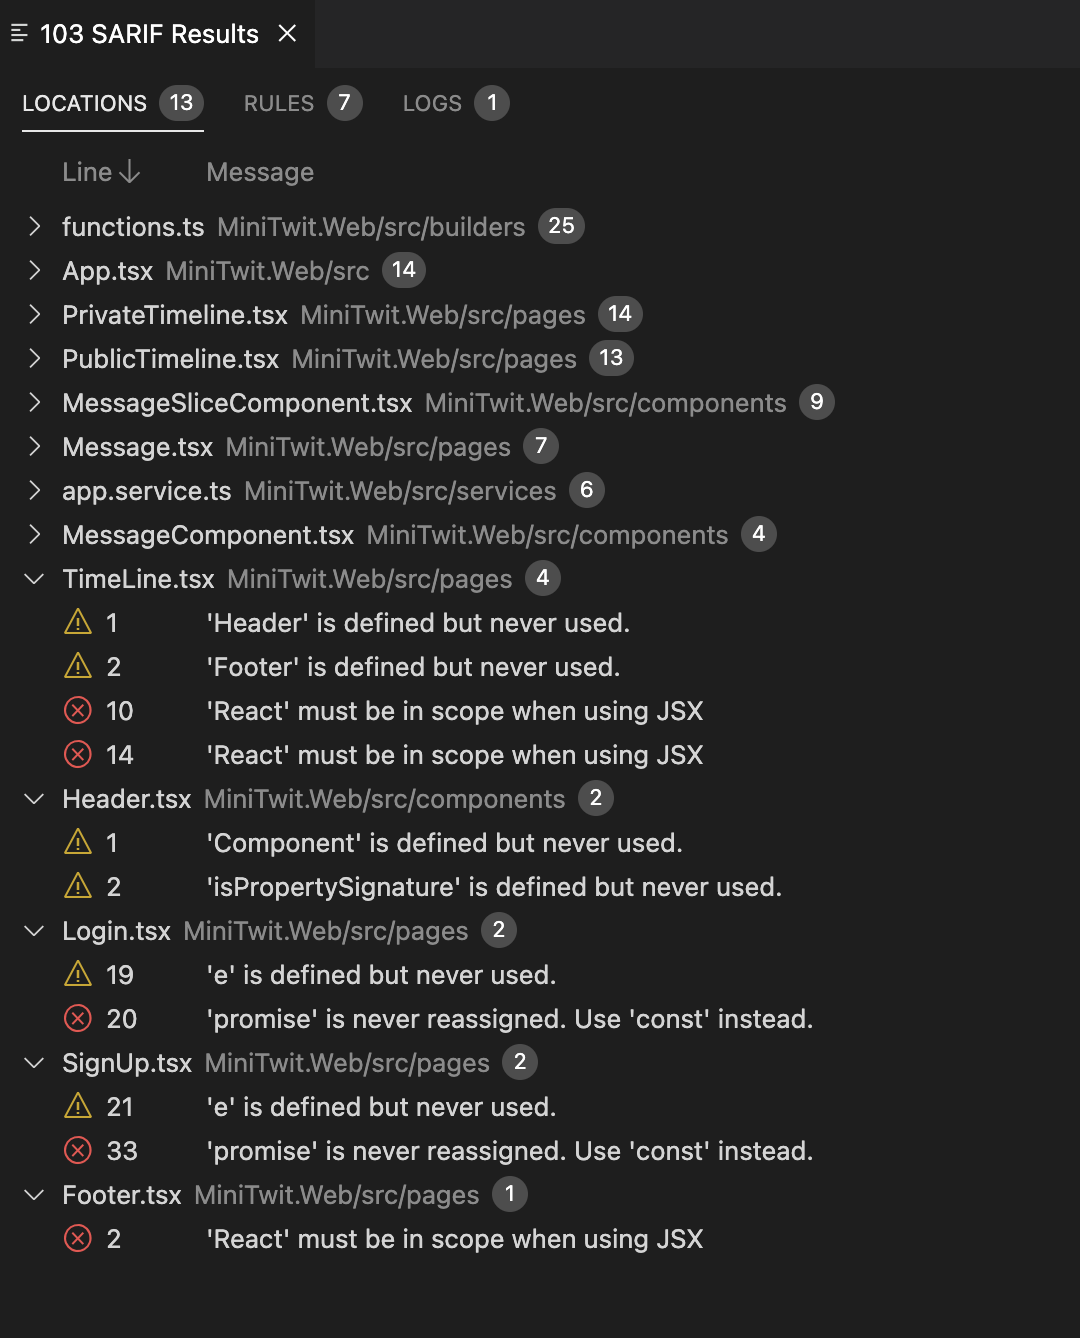
\includegraphics[width=10cm]{Eslint_report.png}
    \caption{Eslint scan - Report}
    \label{fig:my_label}
\end{figure}

\subsection{snyk-security.yml}

\begin{figure}[H]
    \centering
    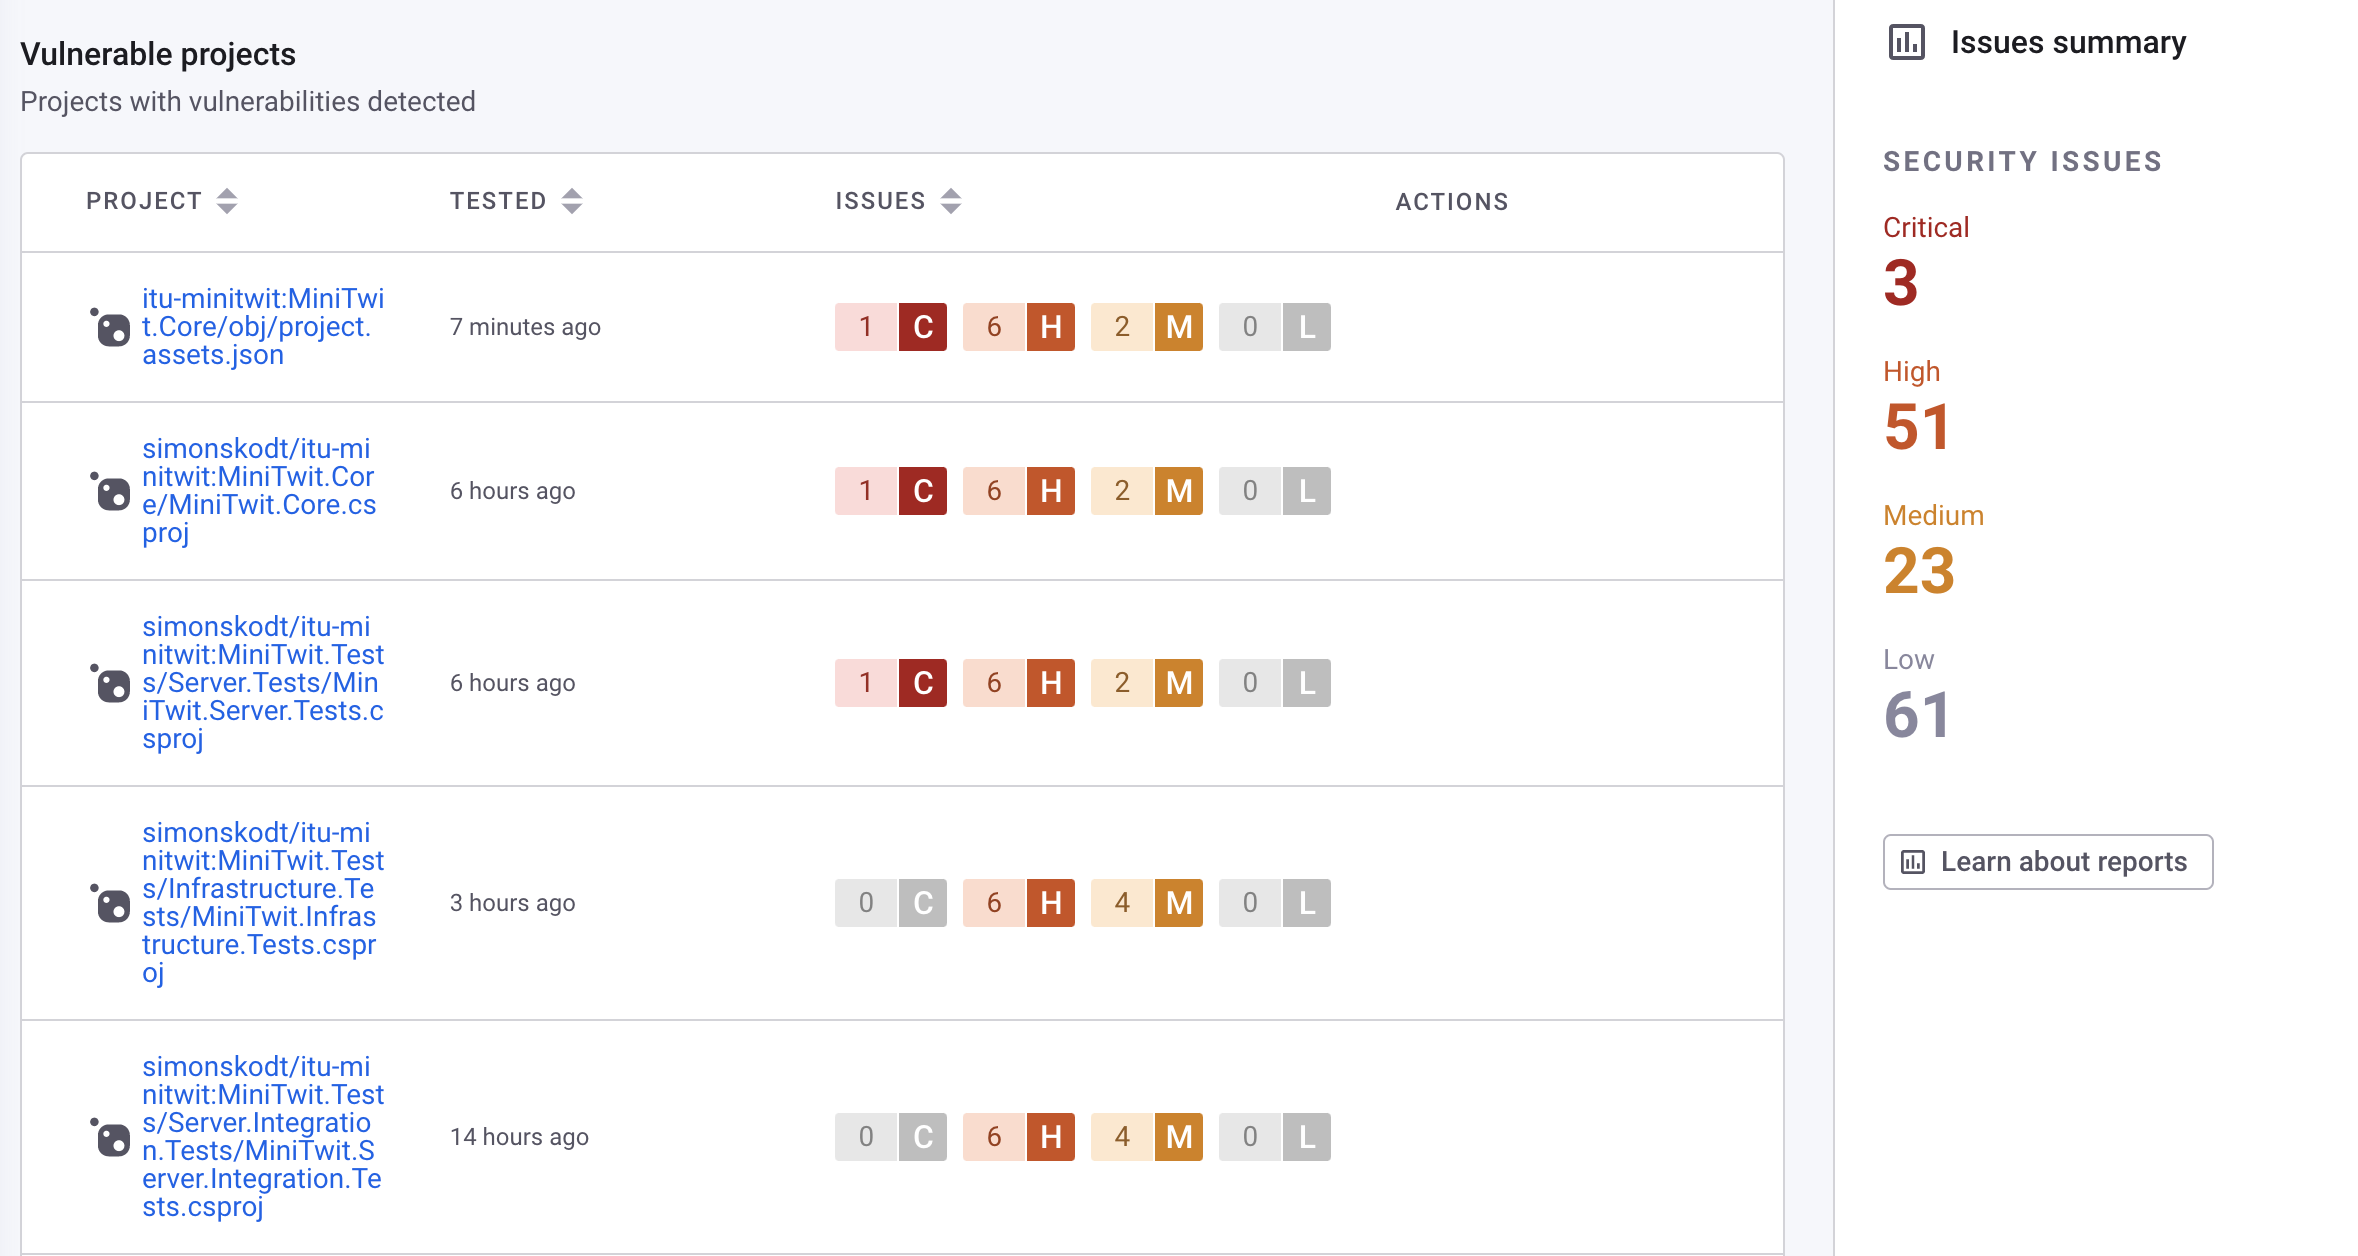
\includegraphics[width=10cm]{Snyk_report.png}
    \caption{Snyk Security - Report}
    \label{fig:my_label}
\end{figure}

\subsection{SonarCloud \& CodeClimate}
Integration with sonarcloud and codeclimate

\begin{figure}[H]
    \centering
    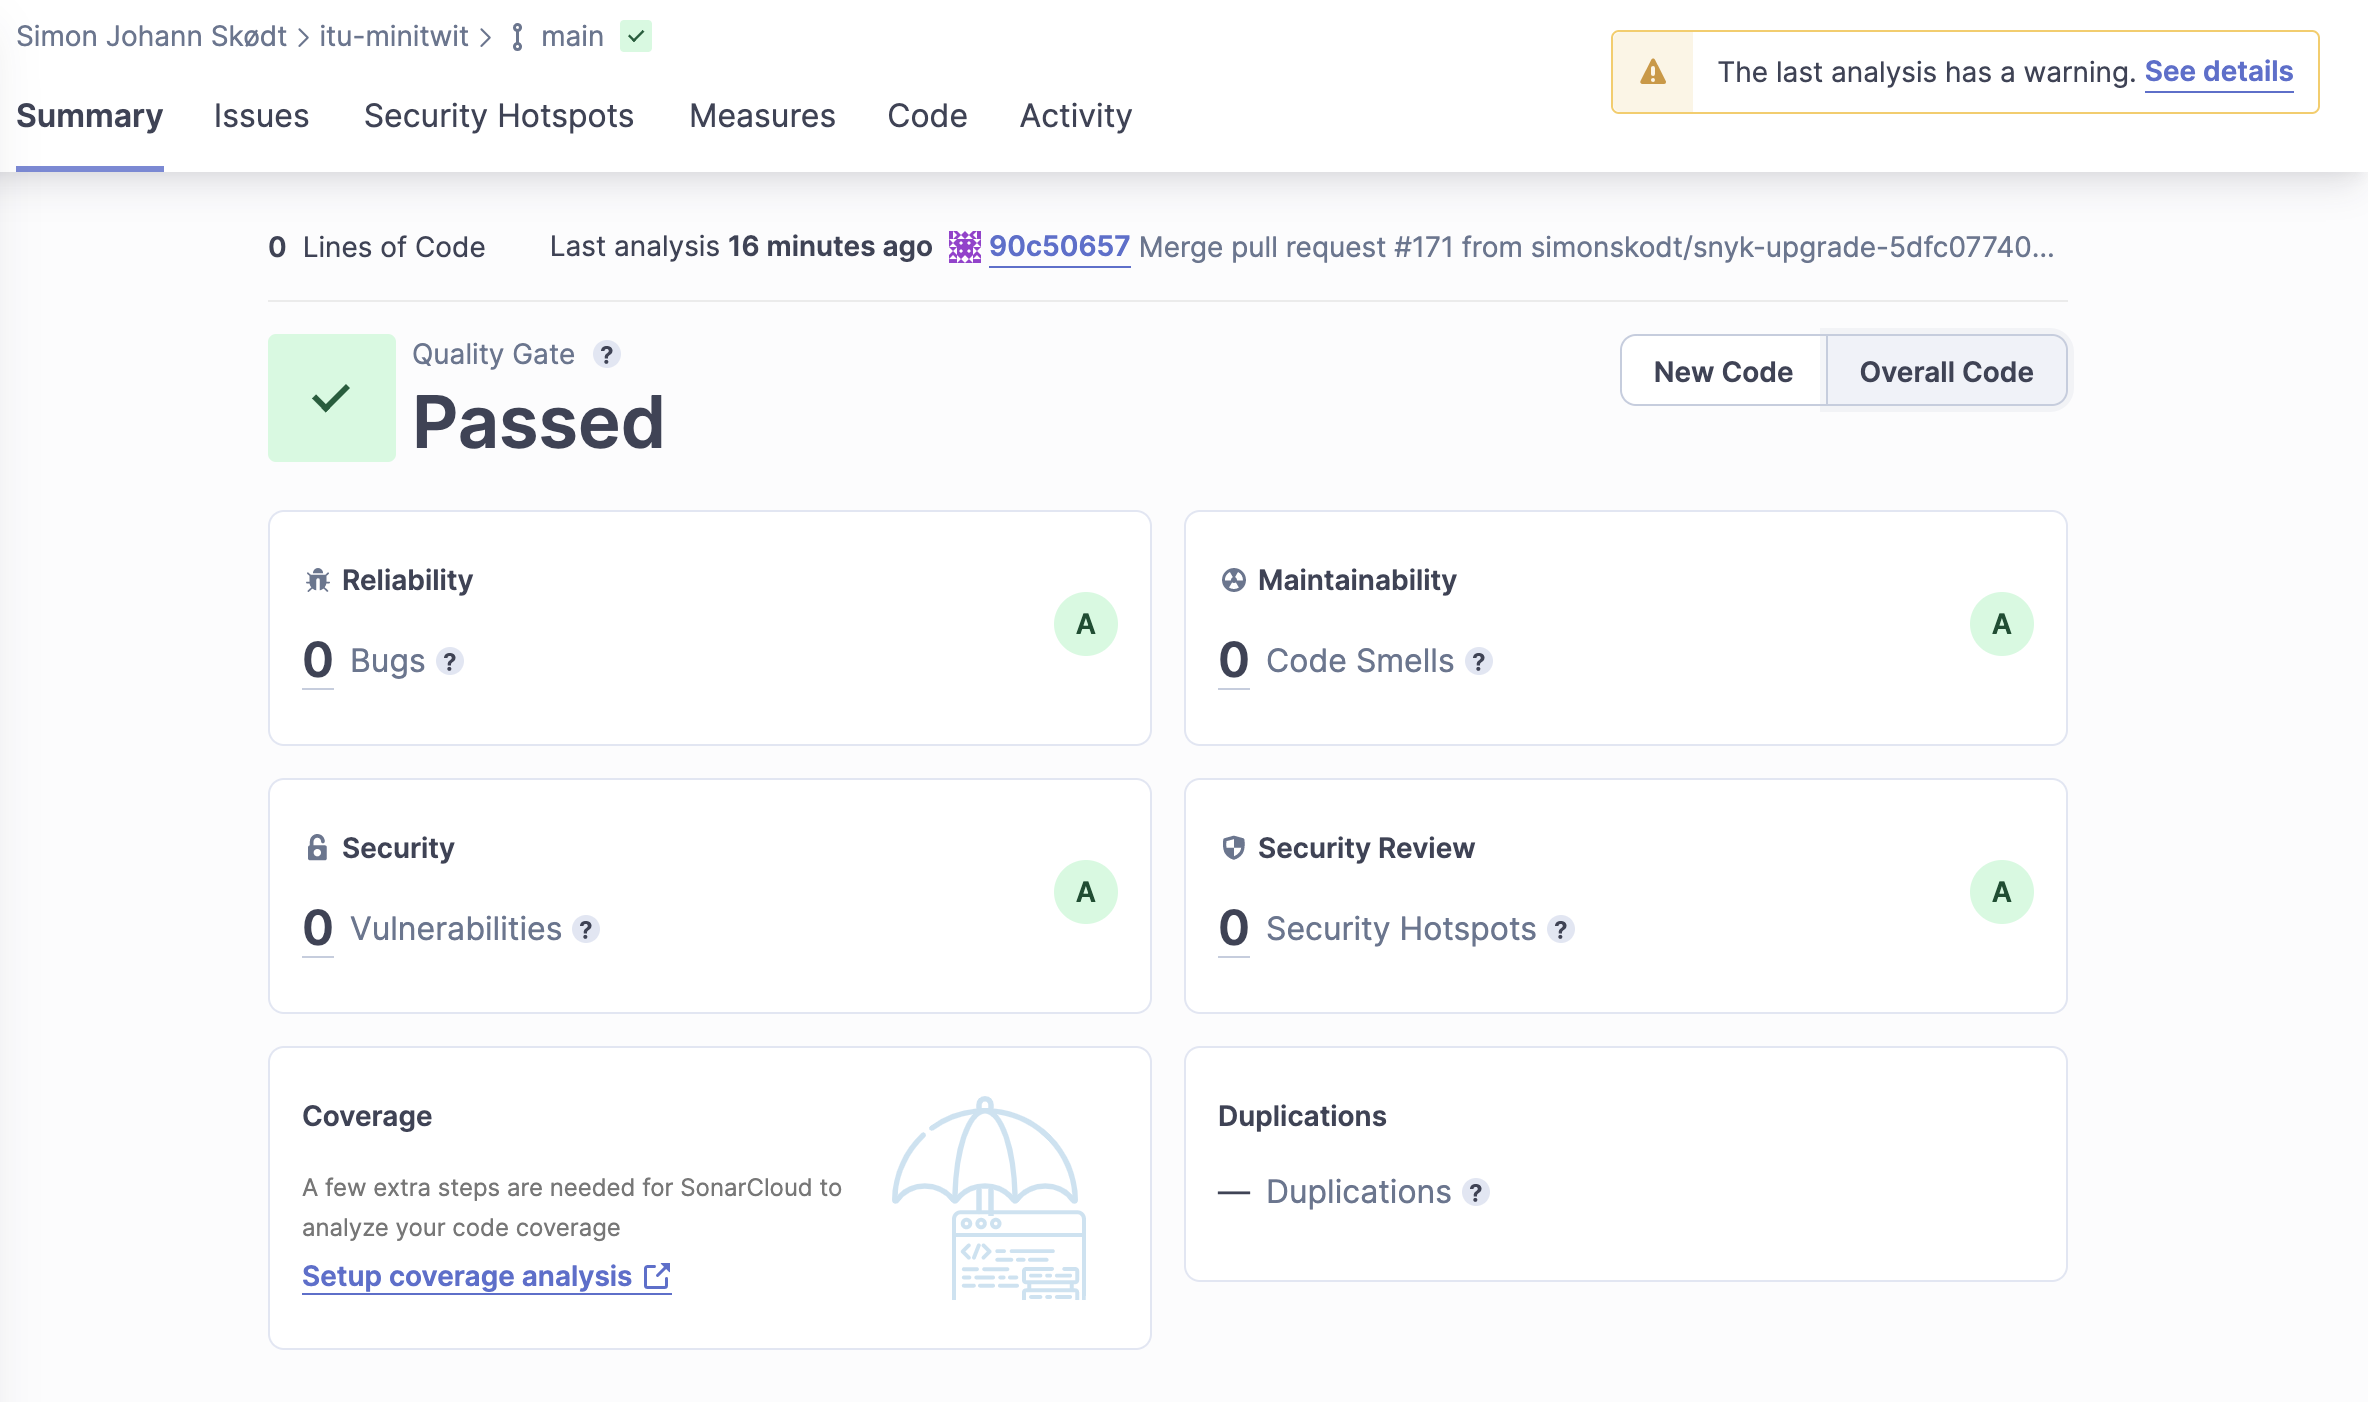
\includegraphics[width=10cm]{Sonar_cloud.png}
    \caption{Sonar Cloud - Report}
    \label{fig:my_label}
\end{figure}

\begin{figure}[H]
    \centering
    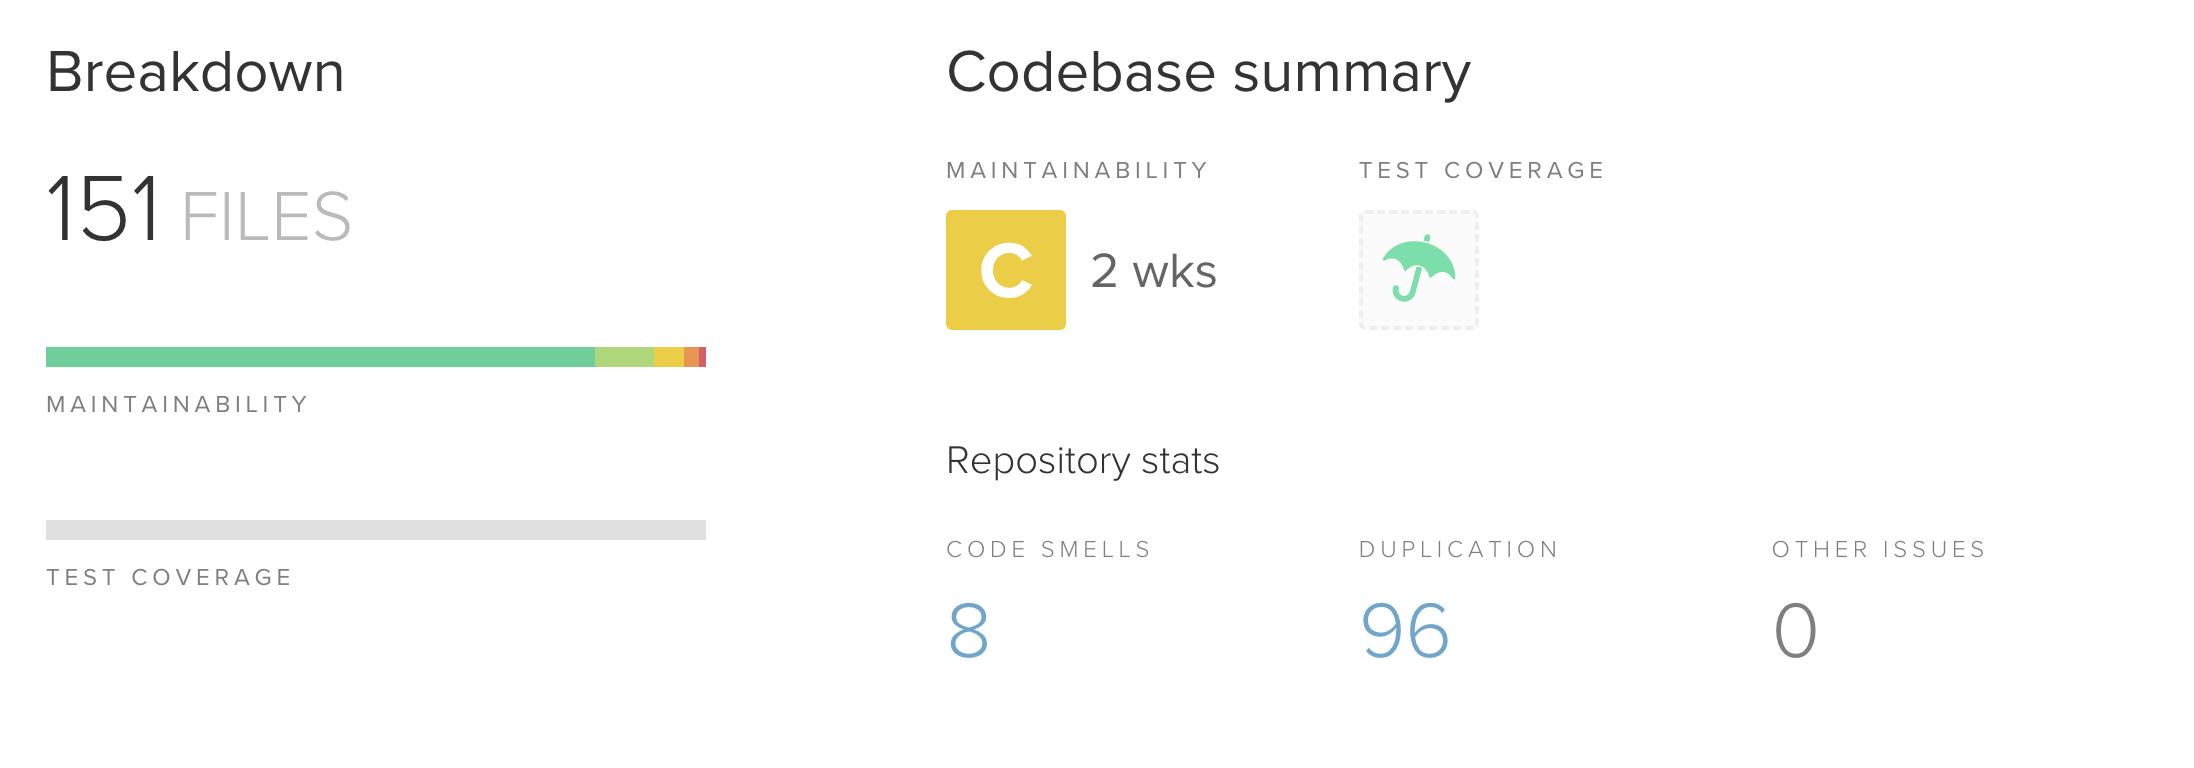
\includegraphics[width=10cm]{Code_climate.png}
    \caption{Code Climate - Report}
    \label{fig:my_label}
\end{figure}

\subsection{continuous-deployment.yml}
Deploytment pipeline (only on push)

\section{Repository Organisation}

\section{Branching Strategy}

\section{Monotoring}

\section{Logging}

\section{Security}

\section{Scaling and Load Balancing}